\title{SABER}
\author{
	dtConfect
	\and
	bombpersons
	}
\date{\today}

\documentclass[12pt,final,twocolumn]{article}

\usepackage{lipsum}											%Lorem Ipsum

\usepackage{graphicx}										%Graphics for images as figures
\usepackage[pdfborder={0 0 0}]{hyperref}
\usepackage{url}											%URL formatting
\usepackage{hyphenat}										%Allow \nohyphens{(text block)}.


% DOCUMENT ENTRY POINT
\begin{document}


%Title page
%\maketitle
\maketitle

\begin{abstract}
The abstract text goes here.
\lipsum[1-6]
\end{abstract}

\section{Introduction}
Here is the text of your introduction.
\lipsum[1-6]

\begin{equation}
    \label{simple_equation}
    \alpha = \sqrt{ \beta }
\end{equation}

\subsection{Subsection Heading Here}
Write your subsection text here.
\lipsum[1-6]

\begin{figure}
    \centering
    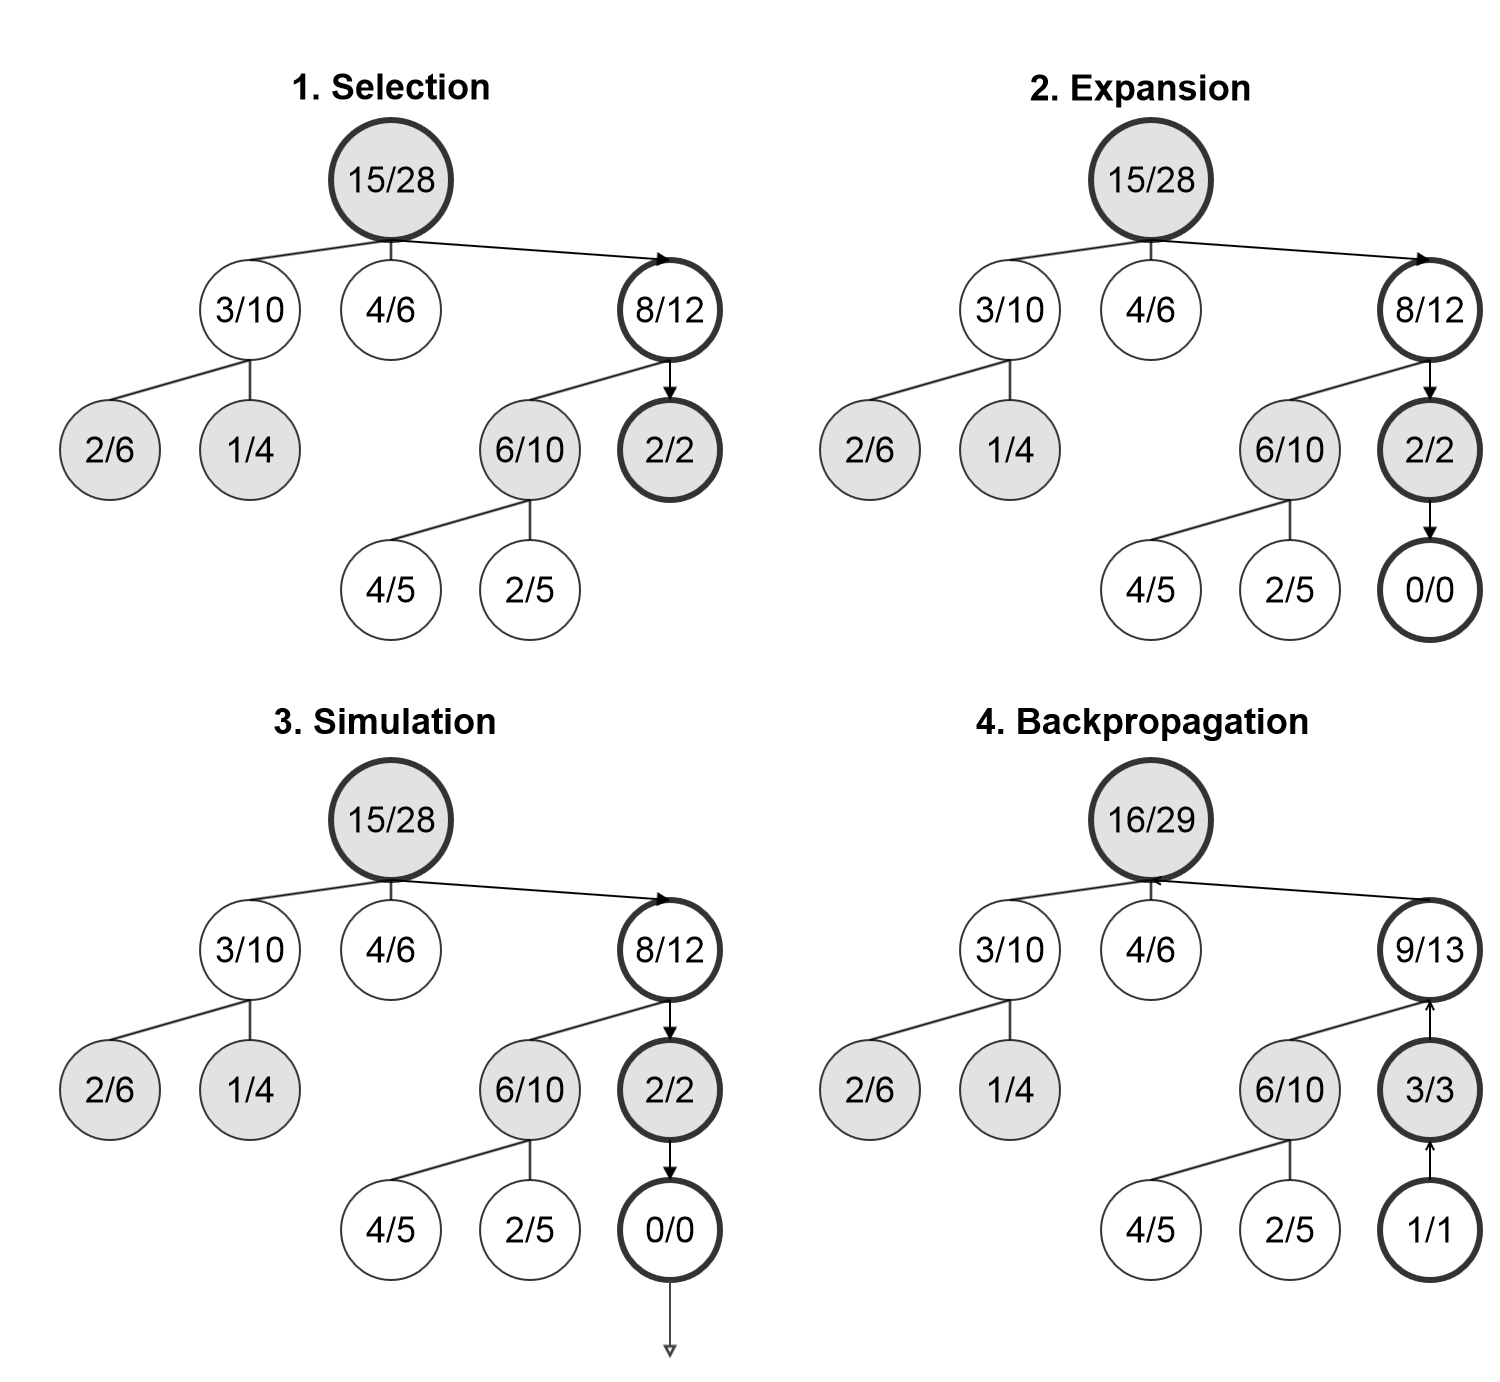
\includegraphics[width=3.0in]{img/test_fig}
    \caption{Simulation Results}
    \label{simulationfigure}
\end{figure}

\section{Conclusion}
Write your conclusion here.
\lipsum[1-6]

\end{document}